% ===========================================================================
% Section 4 -- Initial computational experiments and bottleneck analysis
% ===========================================================================

The three formulations were run on the 76 instances of Section~\ref{sec:suite}
(36 of the scale suite, 30 of the factor suite, 10 from the OR-Library) with
the setup of Section~\ref{sec:setup}: 228 runs, about 1.7 hours of wall-clock
time with five runs in parallel. The raw data are in
\texttt{results/raw/baseline.csv}; the tables and the figure of this section
are generated from that file by \texttt{src/analyze\_baseline.py}.

\paragraph{Correctness.} All 189 solutions returned by the solver were
accepted by the validator. Three (CF-M) incumbents at the time limit
(\texttt{scale\_n150\_s2}, \texttt{scale\_n150\_s3}, \texttt{csp100}) were
first flagged because the reported cost was higher than the cost of the
decoded shifts. In these solutions some employees have $y_k=1$ but no duty.
Constraints $x_{ik}\le y_k$ allow this, and it is never optimal, but an
incumbent found early may contain it. The decoded shifts are feasible; the
idle employees add $1.2$--$5.2$ to the cost. The runner now validates the
decoded shifts at their own cost and records the idle cost separately.

\subsection{Results}

\paragraph{Scalability.} Table~\ref{tab:base-scale} and
Figure~\ref{fig:base-scale} show the scale suite. All three models solve
every instance with $n\le 25$. (AF) is the first to fail: it solves all seeds
only up to $n=25$, no instance with $n\ge 40$, and for $n\ge 80$ it does not
even finish the root node, so the solver has no lower bound (gap 100\%). (CF)
solves all seeds up to $n=50$ in a few seconds and stays within 9\% of its
bound at $n=100$. (CF-M) also solves everything up to $n=50$, with a
single exception at $n=40$, but it is 15--30 times slower than (CF) there and
its gap grows faster. Models are \emph{too large} (over 4 million non-zeros)
from $n=150$ for (AF) and (CF), and at $n=200$ for (CF-M), which has half the
constraints of (CF).

\begin{table}[ht]
\centering
\small
\setlength{\tabcolsep}{4.5pt}
\caption{Scale suite: instances solved to optimality (of 3 seeds), mean time
in seconds (300 for unsolved runs) and mean final gap (\%) between incumbent
and solver bound. A gap of 100 means that the root node did not finish, so no
bound was available.}
\label{tab:base-scale}
\begin{tabular}{rrrrrrrrrr}
\toprule
 & \multicolumn{3}{c}{(AF)} & \multicolumn{3}{c}{(CF)} & \multicolumn{3}{c}{(CF-M)} \\
\cmidrule(lr){2-4} \cmidrule(lr){5-7} \cmidrule(lr){8-10}
$n$ & solved & time & gap & solved & time & gap & solved & time & gap \\
\midrule
10 & 3/3 & 0 & 0.0 & 3/3 & 0 & 0.0 & 3/3 & 0 & 0.0 \\
15 & 3/3 & 1 & 0.0 & 3/3 & 0 & 0.0 & 3/3 & 0 & 0.0 \\
20 & 3/3 & 4 & 0.0 & 3/3 & 0 & 0.0 & 3/3 & 1 & 0.0 \\
25 & 3/3 & 18 & 0.0 & 3/3 & 0 & 0.0 & 3/3 & 1 & 0.0 \\
30 & 2/2 & 35 & 0.0 & 3/3 & 4 & 0.0 & 2/2 & 9 & 0.0 \\
40 & \multicolumn{3}{c}{too large} & 1/1 & 1 & 0.0 & 1/1 & 54 & 0.0 \\
\bottomrule
\end{tabular}

\end{table}

\begin{figure}[ht]
\centering
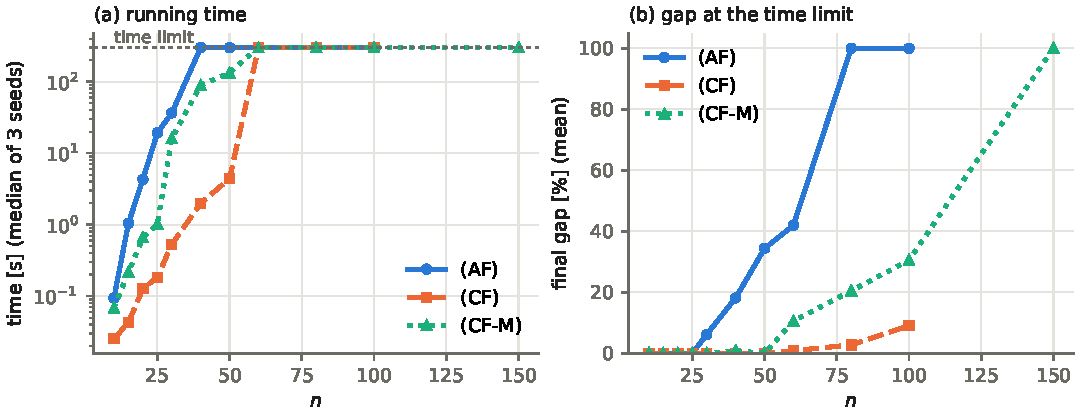
\includegraphics[width=\textwidth]{figures/base_scale}
\caption{Scale suite: (a) running time and (b) final gap as functions of the
number of duties $n$.}
\label{fig:base-scale}
\end{figure}

\paragraph{Formulation strength.} Table~\ref{tab:base-bounds} compares the
bounds with the proven optimum on the 47 transitive instances solved by some
model. The results confirm the theory of Section~\ref{sec:properties}. The LP
relaxation of (AF) is the strongest (19.6\% below the optimum), and the LP of
(CF) and (CF-M) is weak (30.5\%; the two LPs coincide, because spread
constraints are not binding in the LP). The \emph{root} bound, after HiGHS's
presolve and cutting planes, shows a different picture. For (CF) the root gap
drops to 0.8\%, and 40 of its 50 optimal runs need no branching. The
conflict constraints $x_{ik}+x_{jk}\le y_k$ form cliques of pairwise
conflicting duties, and the solver's clique cuts recover what the LP misses.
The big-$M$ spread constraints of (CF-M) do not have this structure: its root
gap stays at 5.5\%, and its solved runs need a median of 1111 nodes. (AF)
improves least at the root (from 19.6\% to 12.2\%). Its LP is slow
(Table~\ref{tab:base-size}), which leaves little time for the cut rounds.

\begin{table}[ht]
\centering
\small
\caption{Bound quality on the transitive instances with a known optimum
$z^*$: mean LP gap $(z^*-z_{\mathrm{LP}})/z^*$ and root gap
$(z^*-z_{\mathrm{root}})/z^*$ (one (AF) run whose root did not finish is
excluded from the root mean), median nodes of the solved runs, runs solved.}
\label{tab:base-bounds}
\begin{tabular}{lrrrrr}
\toprule
Model & instances & LP gap \% & root gap \% & nodes (solved) & solved \\
\midrule
(AF) & 14 & 21.8 & 4.1 & 1 & 14 \\
(CF) & 16 & 34.0 & 0.8 & 1 & 16 \\
(CF-M) & 15 & 34.8 & 1.2 & 1 & 15 \\
\bottomrule
\end{tabular}

\end{table}

\paragraph{Model size and LP time.} Table~\ref{tab:base-size} shows two
typical instances. (AF) has about 15 times more variables than (CF), but
very few rows. Its LP is highly degenerate: the $|\K|$ copies of each arc
are identical, so the simplex method makes many moves that do not change the
objective. At $n=40$ HiGHS needs 23\,s for the LP of (AF), against 0.3\,s
for (CF). At $n=100$ the (AF) LP alone does not finish in 60\,s (14 runs out
of 64). (CF) grows in the other direction: its rows are the conflict
constraints, $O(|\K|\,n^2)$ of them, and this is what makes it too large at
$n=150$.

\begin{table}[ht]
\centering
\small
\caption{Model size and time for the LP relaxation (instances
\texttt{scale\_n040\_s1} and \texttt{scale\_n100\_s1}; pool sizes
$U_{\mathrm F}+U_{\mathrm H}=48$ and $110$).}
\label{tab:base-size}
\begin{tabular}{@{}lrrrrrrrr@{}}
\toprule
& \multicolumn{4}{c}{$n=40$} & \multicolumn{4}{c}{$n=100$} \\
\cmidrule(lr){2-5}\cmidrule(lr){6-9}
Model & vars & rows & non-zeros & LP [s] & vars & rows & non-zeros & LP [s] \\
\midrule
(AF)   & 28\,464 & 2\,104  & 111\,936 & 23.3 & 366\,630 & 11\,430  & 1\,455\,520 & $>60$ \\
(CF)   & 1\,968  & 29\,830 & 91\,194  & 0.3  & 11\,110  & 446\,091 & 1\,348\,753 & 18.0 \\
(CF-M) & 2\,064  & 18\,712 & 54\,000  & 0.3  & 11\,330  & 233\,190 & 688\,050    & 13.1 \\
\bottomrule
\end{tabular}
\end{table}

\paragraph{Primal side.} The solver often finds poor solutions on large
instances. In 14 of the 49 (AF) runs that hit the time limit, the incumbent
is \emph{worse} than the greedy solution used to size the pool. Examples are
$62.8$ against $42.0$ at $n=100$, and $88.8$ against $52.6$ on
\texttt{csp150}. The same happens in 4 of 21 (CF-M) runs, and one (CF-M) run at
$n=100$ ends with no solution at all. (CF) is never worse than its greedy.
The greedy itself is on average 10\% (at most 28\%) above the optimum.

\paragraph{Instance factors.} Table~\ref{tab:base-factor} varies one generator
parameter at a time on $n=40$. (AF) fails on every variant except one sparse
instance (arc\_drop $0.6$), because its size depends on the number of arcs.
For (CF) and (CF-M) a longer total time ($T=960$) and short duties make the
problem easier. A flat demand profile and long duties make (CF) about six
times slower. A plausible reason is that a flat profile has fewer overlapping
duties, so the conflict cliques are smaller. With long duties the working-time
limit binds, and the conflict constraints do not express it. The
strongest effect comes from removing arcs (arc\_drop). The graph is then no
longer transitive and (CF) is a restriction (Remark after
Proposition~\ref{prop:cf}). It becomes slower, and its result can be wrong. On
\texttt{fac\_arc\_drop-0.6\_s3}, (AF) proves an optimum of $16.0$, while (CF)
cannot go below its bound of $16.2$.

\begin{table}[ht]
\centering
\small
\setlength{\tabcolsep}{4.5pt}
\caption{Factor suite ($n=40$, 3 seeds per variant, one parameter changed
from the default): solved, mean time [s], mean final gap [\%].}
\label{tab:base-factor}
\begin{tabular}{lrrrrrrrrr}
\toprule
 & \multicolumn{3}{c}{(AF)} & \multicolumn{3}{c}{(CF)} & \multicolumn{3}{c}{(CF-M)} \\
\cmidrule(lr){2-4} \cmidrule(lr){5-7} \cmidrule(lr){8-10}
Variant & solved & time & gap & solved & time & gap & solved & time & gap \\
\midrule
default & -- & -- & -- & -- & -- & -- & -- & -- & -- \\
profile-uniform & -- & -- & -- & -- & -- & -- & -- & -- & -- \\
durations-short & -- & -- & -- & -- & -- & -- & -- & -- & -- \\
durations-long & -- & -- & -- & -- & -- & -- & -- & -- & -- \\
travel-low & -- & -- & -- & -- & -- & -- & -- & -- & -- \\
travel-high & -- & -- & -- & -- & -- & -- & -- & -- & -- \\
T-960 & -- & -- & -- & -- & -- & -- & -- & -- & -- \\
T-600 & -- & -- & -- & -- & -- & -- & -- & -- & -- \\
arc\_drop-0.3 & -- & -- & -- & -- & -- & -- & -- & -- & -- \\
arc\_drop-0.6 & -- & -- & -- & -- & -- & -- & -- & -- & -- \\
\bottomrule
\end{tabular}

\end{table}

\paragraph{OR-Library.} The OR-Library graphs are not transitive, so only
(AF) is exact on them (Table~\ref{tab:base-orlib}). (AF) solves none of them:
it reaches a gap of 21\% on \texttt{csp50}. From \texttt{csp100} on, its
incumbents are much worse than the greedy, and from \texttt{csp150} it has no
bound. From \texttt{csp250} the model is too large. The restriction (CF) also
pays for non-transitivity before any optimisation. The greedy limited to
pairwise-compatible shifts (greedy$^{\mathrm{pw}}$) is 15--26\% more expensive
than the general one. The (CF) bounds (20.0 and 31.6) bound only the
restriction, not the problem, and on \texttt{csp100} its best solution (38.4)
is worse than the general greedy (33.8). None of the baseline models can
handle realistic OR-Library sizes.

\begin{table}[ht]
\centering
\small
\setlength{\tabcolsep}{4pt}
\caption{OR-Library instances ($W=480$, $T=720$). LB is the combinatorial
lower bound of Section~\ref{sec:inst-stats}; greedy is the general greedy and
greedy$^{\mathrm{pw}}$ the pairwise one used for (CF). The (CF) bound is a
bound of the restriction only. ``none'': the root node did not finish;
``large'': over 4 million non-zeros.}
\label{tab:base-orlib}
\begin{tabular}{rrrrrrrr}
\toprule
 & & & \multicolumn{3}{c}{(AF)} & \multicolumn{2}{c}{(CF) restriction} \\
\cmidrule(lr){4-6}\cmidrule(lr){7-8}
$n$ & LB & greedy & obj & bound & status & obj & bound \\
\midrule
\bottomrule
\end{tabular}

\end{table}

\subsection{Bottleneck analysis}
\label{sec:bottlenecks}

From these results we identify five bottlenecks. Each suggests an improvement
for Section~\ref{sec:improvements}.

\begin{enumerate}[label=\textbf{B\arabic*.}]
  \item \textbf{Size of the compact models.} Both exact formulations index
    every variable by employee, so their size is $|\K|$ times that of a single
    shift: $O(|\K|\,|\A|)$ for (AF) and $O(|\K|\,n^2)$ for (CF). With
    $|\K|=U_{\mathrm F}+U_{\mathrm H}$ up to $2.7\,\bar z$ this limits us to
    $n\le 100$, while the
    OR-Library goes up to $n=500$. \emph{Hypothesis:} a formulation without
    employee index, the set partitioning model (SP) of
    Section~\ref{sec:sp} solved by column generation, removes this
    dependence. Smaller pools, from a better heuristic $\bar z$, would help
    the compact models.
  \item \textbf{Symmetry.} Employees of the same type are interchangeable.
    Any solution has $U_{\mathrm F}!\,U_{\mathrm H}!$ copies, and branching on
    one employee's variable does not move the bound. This explains the many
    nodes of (CF-M) and the degenerate LP of (AF). \emph{Hypothesis:}
    symmetry-breaking constraints ($y_k\ge y_{k+1}$, and assigning
    duty~$i$ only to the first $i$ employees) reduce the nodes and the LP
    time. (SP) has no such symmetry.
  \item \textbf{Weak LP relaxation of (CF).} The 30\% LP gap
    (Proposition~\ref{prop:lp-cf}) is closed only by the solver's clique
    cuts, which are generic and become expensive as the number of rows
    grows; at $n=100$ (CF) does not finish the root node. \emph{Hypothesis:}
    replacing the pairwise time conflicts by \emph{maximal clique}
    constraints $\sum_{i\in Q}x_{ik}\le y_k$, one per maximal set $Q$ of
    pairwise overlapping duties, gives a stronger and much smaller model.
    The time-conflict graph is an interval graph, so it has at most $n$
    maximal cliques and they are found by one sweep over the start times.
  \item \textbf{Poor primal solutions.} The solver often ends with an
    incumbent worse than a simple greedy, or with none. \emph{Hypothesis:}
    passing the greedy as a starting solution (MIP start), and improving it
    with a local search, gives every run a good upper bound from the
    start. It also lets the solver prune more nodes. Removing idle employees
    from the incumbents costs nothing and is always valid.
  \item \textbf{Non-transitive graphs.} (CF) is fast but only a restriction
    when the triangle inequality fails, which is the case on the OR-Library
    and on the arc\_drop instances, and (AF) is exact but too large there.
    \emph{Hypothesis:} (SP), whose columns are paths in $G$, is exact on any
    graph, so it removes this trade-off.
\end{enumerate}

Further, smaller improvements: all costs are multiples of $0.2$, so the
objective scaled by $5$ is integer and any bound $z_{\mathrm{LB}}$ can be
rounded up to $\lceil 5z_{\mathrm{LB}}\rceil/5$. This closes the final gaps
of many time-limit runs at little cost. A second solver (Gurobi, with an
academic licence) would show how much of the difference between the models
is due to HiGHS.
